\chapter{Schmale Flüsse mit Zurücksetzen}\label{sec-thin-flows}
\newcommand*{\PlH}{\makebox[1ex]{\textbf{$\cdot$}}}

\section{Definition und Eigenschaften}

Der Abschnitt beginnt mit der Einführung einer neuen Klasse statischer Flüsse:

\begin{definition}[$s$-Fluss]
	Ein $b$-Fluss $f$ in einem Graphen $(V, E)$ heißt \emph{$s$-Fluss} für ein $s\in V$, falls $b_v\leq 0$ für alle $v\in V\setminus \{ s \}$ gilt.
	Dabei bezeichnet $b_s$ den \emph{Wert von $f$}. 
\end{definition}

\begin{definition}[Netzwerk mit Zurücksetzen]
	Ein \emph{Netzwerk mit Zurücksetzen auf $E_1$ und Ursprung $s$} ist ein Tupel $(V, E, u, s, E_1)$, wobei $(V, E, u)$ ein azyklisches Netzwerk ist, in dem der Knoten $s\in V$ jeden anderen Knoten erreicht, und $E_1\subseteq E$ die Menge der \emph{zurücksetzenden Kanten} ist.
\end{definition}

\begin{definition}[Auslastung]
	Sei ein $s$-Fluss $f$ in einem Netzwerk mit Zurücksetzen auf $E_1$ und Ursprung $s$ gegeben.
	Dann ist die \emph{Auslastung einer Kante} gegeben durch $f_e/u_e$.
	Die \emph{Auslastungsübertragung einer Kante $vw$} ist gegeben durch \[ \rho_{vw}(l_v, f_{vw}) := \begin{cases}
		\max\{ l_v, f_{vw} / u_{vw} \}, & \text{falls $vw\notin E_1$,}\\
		f_{vw} / u_{vw}, & \text{falls $vw\in E_1$.}
	\end{cases}
	\]
	Die \emph{Auslastung eines $s$-$v$-Pfades $P=(e_1,\dots,e_k)$} ist dann gegeben durch die Verkettung $(\rho_{e_k}(\PlH, f_{e_k})\circ \dots \circ \rho_{e_1}(\PlH, f_{e_1}))(0)$.
	Die zu $f$ \emph{zugehörige Knotenauslastung $l\in\R_{\geq 0}^V$} sei dann für einen Knoten $v\in V$ festgelegt durch die minimale Auslastung eines $s$-$v$-Pfades.
\end{definition}

Betrachtet man einen $s$-$v$-Pfad $P=(e_1, \dots, e_k)$, der Kanten aus $E_1$ enthält, so ist die Auslastung von $P$ gerade $\max_{j=i}^k f_{e_j}/u_{e_j}$, wobei $e_i$ die letzte Kante des Pfades in $E_1$ ist.
Daher nennt man die Kanten in $E_1$ die zurücksetzenden Kanten, da sie die Auslastung eines vorangegangen Pfades auf ihre eigene zurücksetzen.

\begin{proposition}\label{prop-congestion-labels-dijkstra}
	Die Knotenauslastungen eines $s$-Flusses $f$ sind gegeben durch die eindeutige Lösung $(\tilde{l}_v)_{v\in V}$ des Gleichungssystems
	\[
	\tilde{l}_w = \begin{cases}
		0, & \text{falls $w=s$,}\\
		\min_{vw\in \delta^-(w)} \rho_{vw}(\tilde{l}_v, f_{vw}), & \text{sonst.}
	\end{cases}
	\]
\end{proposition}
\begin{proof}
	Die Existenz einer Lösung folgt aus der Azyklizität des Netzwerks und wegen der Erreichbarkeit jedes Knotens von $s$ aus.
	
	Sei also $\tilde{l}\in\R_{\geq 0}^V$ die Lösung des Gleichungssystems.
	Der Teilgraph $(V, E')$ mit \[
	E':= \left\{ vw\in E ~\middle\vert~ \rho_{vw}(\tilde{l}_v, f_{vw}) = \min_{uw\in\delta^-(w)}  \rho_{uw}(\tilde{l}_u, f_{uw}) \right\}
	\]
	ebenfalls azyklisch und jeder Knoten ist von $s$ aus erreichbar.
	Man zeige $l_w = \tilde{l}_w$ durch eine Induktion über die Distanz von $w$ zu $s$ bezüglich der Anzahl an Kanten.
	Für $w=s$ gilt offenbar $l_s = 0$.
	Sei nun ein $s$-$w$-Pfad $P$ gegeben, seien $vw$ die letzte Kante und $Q$ das restliche Anfangsstück dieses Pfades.
	Nach Induktionsvoraussetzung ist die Auslastung von $Q$ mindestens $\tilde{l}_v$.
	Daher ist die Auslastung von $P$ mindestens $\rho_{vw}(\tilde{l}_v, f_{vw})$ aufgrund der Monotonie von $\rho_{vw}(\PlH, f_{vw})$, wodurch $l_v \geq \tilde{l}_v$ folgt.
	Außerdem hat ein $s$-$v$-Pfad $P$, der in $(V, E')$ verläuft, hat Auslastung $\tilde{l}_v$.
	Da solch ein Pfad existiert, gilt also $l_v \leq \tilde{l}_v$.
\end{proof}

\newcommand{\problemThinFlow}{\textsc{ThinFlow}}
\begin{definition}[Schmaler Fluss]
	Seien ein $s$-Fluss $f$ in einem Netzwerk mit Zurück\-setzen auf $E_1$ und Ursprung $s$ sowie die durch $f$ induzierten Knotenauslastungen $l$ gegeben.
	Der Fluss $f$ heißt \emph{schmaler Fluss mit Zurücksetzen auf $E_1$}, falls die Auslastung jedes $s$-$v$-Pfades mit positivem Fluss $l_v$ beträgt.
	
	Dabei nennt man das Tupel $(V, E, u, s, b, E_1)$ eine \emph{Instanz des $\problemThinFlow$ Problems}.
\end{definition}

Insbesondere ist bei einem schmalen Fluss die Knotenauslastung $l_v$ eines Knotens $v$ gerade die Auslastung eines jeden $s$-$v$-Pfades mit positivem Fluss und $0$, falls kein solcher existiert.

\begin{remark}
	Ronald Koch betrachtet in~\cite{Koch2012} allgemeinere schmale Flüsse: Dort ist das zugrundeliegende Netzwerk nicht als azyklisch vorausgesetzt.
	Diese Einschränkung wird hier im Sinne von~\cite{Cominetti2015} beibehalten.
\end{remark}

\begin{figure}
	\centering
	\newcommand{\newnode}[4]{\node[lul] (#1) at #2 {#3 \\[0.5em] #4};}
	\begin{subfigure}{\textwidth}
		\begin{tikzpicture}[lul/.style={draw,
			ellipse,
			align=center,
			inner sep=0pt,
			outer sep=4pt,
			text width=7mm,
			minimum height=1.5cm
		}]
		
		\newnode{0}{(0,2)}{$a$}{$32$}
		\newnode{1}{(3,2)}{$b$}{$0$}
		\newnode{2}{(5,0)}{$c$}{$-2$}
		\newnode{3}{(7,2)}{$d$}{$-12$}
		\newnode{4}{(10,3)}{$e$}{$-2$}
		\newnode{5}{(10,1)}{$f$}{$0$}
		\newnode{6}{(13,2)}{$g$}{$-16$}
		
		\begin{scope}[-Latex]
		\path [-Latex] (0) edge node[above] {$4$} (1);
		\path [-Latex] (0) edge[bend right] node[above] {$4$} (2);
		\path [-Latex] (0) edge[bend left] node[above] {$4$} (4);
		\path [-Latex] (1) edge node[right] {$2$} (2);
		\path [-Latex] (1) edge node[above] {$2$} (3);
		\path [-Latex] (2) edge node[left] {$2$} (3);
		\path [-Latex] (3) edge node[above] {$1$} (4);
		\path [-Latex] (3) edge node[above] {$2$} (5);
		\path [-Latex] (4) edge node[above] {$1$} (6);
		\path [-Latex] (5) edge node[above] {$1$} (6);
		\end{scope}
		\end{tikzpicture}
		\subcaption{Der Ursprungsgraph. Die Kanten $e$ sind mit Kapazitäten $u_e$ und die Knoten $v$ mit einem Bezeichner $v$ und einer Balance $b_v$ beschriftet.}
	\end{subfigure}
	\par\bigskip
	\begin{subfigure}{\textwidth}
		\begin{tikzpicture}[lul/.style={draw,
			ellipse,
			align=center,
			inner sep=0pt,
			outer sep=4pt,
			text width=7mm,
			minimum height=1.5cm
		}]
		
		\newnode{0}{(0,2)}{$a$}{$0$}
		\newnode{1}{(3,2)}{$b$}{$2{,}75$}
		\newnode{2}{(5,0)}{$c$}{$2{,}75$}
		\newnode{3}{(7,2)}{$d$}{$5$}
		\newnode{4}{(10,3)}{$e$}{$2{,}5$}
		\newnode{5}{(10,1)}{$f$}{$5$}
		\newnode{6}{(13,2)}{$g$}{$8$}
		
		\begin{scope}[-Latex]
		\path [-Latex] (0) edge node[above] {$11/4$} (1);
		\path [-Latex] (0) edge[bend right] node[above] {$11/4$} (2);
		\path [-Latex] (0) edge[bend left] node[above] {$10/4$} (4);
		\path [-Latex] (1) edge node[right] {$1/2$} (2);
		\path [-Latex] (1) edge node[above] {$10/2$} (3);
		\path [-Latex] (2) edge node[left] {$10/2$} (3);
		\path [-Latex] (3) edge node[above] {$0/1$} (4);
		\path [-Latex] (3) edge node[above] {$8/2$} (5);
		\path [-Latex] (4) edge node[above] {$8/1$} (6);
		\path [-Latex] (5) edge node[above] {$8/1$} (6);
		\end{scope}
		\end{tikzpicture}
		\subcaption{Ein schmaler Fluss $f$ ohne Zurücksetzen.}
		\label{subfig-thin-flow-without-resetting}
	\end{subfigure}
	\par\bigskip
	\begin{subfigure}{\textwidth}
		\begin{tikzpicture}[lul/.style={draw,
			ellipse,
			align=center,
			inner sep=0pt,
			outer sep=4pt,
			text width=7mm,
			minimum height=1.5cm
		},
		scale=1]
		
		\newnode{0}{(0,2)}{$a$}{$0$}
		\newnode{1}{(3,2)}{$b$}{$3$}
		\newnode{2}{(5,0)}{$c$}{$3$}
		\newnode{3}{(7,2)}{$d$}{$5{,}5$}
		\newnode{4}{(10,3)}{$e$}{$2$}
		\newnode{5}{(10,1)}{$f$}{$5{,}5$}
		\newnode{6}{(13,2)}{$g$}{$8$}
		
		\begin{scope}[-Latex]
		\path [-Latex] (0) edge node[above] {$12/4$} (1);
		\path [-Latex] (0) edge[bend right] node[above] {$12/4$} (2);
		\path [-Latex] (0) edge[bend left] node[above] {$8/4$} (4);
		\path [-Latex] (1) edge node[right] {$1/2$} (2);
		\path [-Latex] (1) edge node[above] {$11/2$} (3);
		\path [-Latex] (2) edge node[left] {$11/2$} (3);
		\path [Square-Latex] (3) edge node[above] {$2/1$} (4);
		\path [-Latex] (3) edge node[above] {$8/2$} (5);
		\path [-Latex] (4) edge node[above] {$8/1$} (6);
		\path [-Latex] (5) edge node[above] {$8/1$} (6);
		\end{scope}
		\end{tikzpicture}
		\subcaption{Ein schmaler Fluss mit Zurücksetzen auf $(d,e)$.}
		\label{subfig-thin-flow-with-resetting}
	\end{subfigure}
\caption{Ein schmaler Fluss einmal ohne Zurücksetzen und einmal mit Zurücksetzen auf $(d,e)$.
	In~\ref{subfig-thin-flow-without-resetting} und~\ref{subfig-thin-flow-with-resetting} hat die Kantenbeschriftung die Form $f_e/u_e$ und in den Knoten steht die Knotenauslastung.}
\end{figure}

\begin{lemma}\label{lemma-thin-flow-t-def}
	Ein $s$-Fluss $f$ in einem Netzwerk mit Zurücksetzen auf $E_1$ und Ursprung $s$ ist genau dann ein schmaler Fluss mit Zurücksetzen auf $E_1$, wenn eine Knotenbewertung $l\in\R_{\geq 0}^V$ existiert, die die folgenden Bedingungen erfüllt:
	\begin{enumerate}[label=(T\arabic*)]
		\item\label{def-thin-flow-source} $l_s = 0$,
		\item\label{def-thin-flow-x-zero} $l_w \leq l_v$, \tabto{4.5cm} für $vw\in E \setminus E_1$ mit $f_{vw}=0$,
		\item\label{def-thin-flow-x-positive} $l_w = \max\{ l_v, f_{vw} / u_{vw} \}$,  \tabto{4.5cm} für $vw\in E\setminus E_1$ mit $f_{vw} > 0$,
		\item\label{def-thin-flow-resetting-edge} $l_w = f_{vw} / u_{vw}$,  \tabto{4.5cm} für $vw\in E_1$,
		\item\label{def-thin-flow-no-resetting-edge} $l_w \geq \min_{vw\in \delta^-(w)} l_v$, \tabto{4.5cm} falls $\delta^-(w)\cap E_1 = \emptyset$.
	\end{enumerate}
	Diese Knotenbewertung stimmt dann mit der Knotenauslastung von $f$ überein.
	Außerdem gelten die Bedingungen~\ref{def-thin-flow-source}, \ref{def-thin-flow-x-zero} und~\ref{def-thin-flow-no-resetting-edge} bereits für die Knotenauslastungen von $f$, falls $f$ nur ein $s$-Fluss ist.
\end{lemma}
\begin{proof}
	Sei $f$ ein schmaler Fluss mit Zurücksetzen auf $E_1$ und sei $l\in\R_{\geq 0}^V$ die Knotenauslastung von $f$.
	Man zeige, dass $l$ die Bedingungen~\ref{def-thin-flow-source}-\ref{def-thin-flow-no-resetting-edge} erfüllt, und benutze dabei die Darstellung aus Proposition~\ref{prop-congestion-labels-dijkstra}.
	Wegen $l_s = 0$ gilt bereits~\ref{def-thin-flow-source}.
	Für eine Kante $vw\in E\setminus E_1$ mit $f_{vw}=0$ gilt $l_w\leq \rho_{vw}(l_v, f_{vw}) = l_v$, wodurch auch~\ref{def-thin-flow-x-zero} folgt.
	Ist $vw\in E$ mit $f_{vw} > 0$, so existiert ein $s$-$w$-Pfad mit positivem Fluss, der die Kante $vw$ benutzt, sodass die Auslastung dieses Pfades $l_w=\rho_{vw}(l_v, f_{vw})$ ist, da der $s$-$v$-Teilpfad die Auslastung $l_v$ besitzt.
	Für $vw\notin E_1$ bedeutet das gerade $l_w = \max\{ l_v, f_{vw}/u_{vw} \}$ also~\ref{def-thin-flow-x-positive}, und für $vw\in E_1$ zeigt das $l_w = f_{vw} / u_{vw}$.
	Für~\ref{def-thin-flow-resetting-edge} bleibt der Fall $f_{vw} = 0$ zu prüfen:
	Dann ist aber $l_w = \min_{uw\in\delta^-(w)} \rho_{uw}(l_u, f_{uw}) = f_{vw} / u_{vw} = 0$.
	Zuletzt betrachte man den Fall, dass $w$ keine eingehende zurücksetzende Kante hat.
	Dann folgt aber bereits $l_w = \min_{vw\in \delta^-(w)} \max\{ l_v, f_{vw} / u_{vw} \} \geq \min_{vw\in\delta^-(w)} l_v$, was auch~\ref{def-thin-flow-no-resetting-edge} impliziert.
	
	Sei nun umgekehrt $l\in\R_{\geq 0}^V$ eine Knotenbewertung, die~\ref{def-thin-flow-source}-\ref{def-thin-flow-no-resetting-edge} erfüllt.
	Man verwende eine Induktion über die Distanz eines Knotens $w$ zu $s$ bezüglich der Kantenzahl, um zu zeigen, dass $l_w$ die Knotenauslastung von  $f$ ist.
	Für $w=s$ gilt $l_s=0$ bereits nach~\ref{def-thin-flow-source}.
	Für $w\neq s$ ist $l_w$ nach~\ref{def-thin-flow-x-zero},~\ref{def-thin-flow-x-positive} und~\ref{def-thin-flow-resetting-edge} eine untere Schranke an $\rho_{vw}(l_v, f_{vw})$ für $vw\in\delta^-(w)$.
	Es bleibt zu zeigen, dass für eine eingehende Kante $vw$ der Wert $\rho_{vw}(l_v, f_{vw})$ auch $l_w$ annimmt:
	Falls eine eingehende Kante $vw\in E_1$ oder eine eingehende Kante $vw$ mit $f_{vw} > 0$ existiert, ist $\rho_{vw}(l_v, f_{vw}) = l_w$ nach~\ref{def-thin-flow-resetting-edge} und~\ref{def-thin-flow-x-positive}.
	Sonst ist $l_w\geq \min_{vw\in \delta^-(w)} l_v = \min_{vw\in \delta^-(w)} \rho_{vw}(l_v', x_{vw}')$ nach~\ref{def-thin-flow-no-resetting-edge}, was die Behauptung zeigt.
	Um zu sehen, dass $f$ nun ein schmaler Fluss mit Zurücksetzen auf $E_1$ ist, genügen die Bedingungen~\ref{def-thin-flow-source}, \ref{def-thin-flow-x-positive} und~\ref{def-thin-flow-resetting-edge}, da dadurch jeder $s$-$v$-Teilpfad eines Pfades mit positivem Fluss gerade Auslastung $l_v$ hat.
\end{proof}

\begin{remark}\label{remark-thin-flow}
	Hier ist, wie in~\cite[Definition~4]{Cominetti2011}, im Vergleich zu~\cite[Definition~6]{Koch2011} die Bedingung~\ref{def-thin-flow-no-resetting-edge} zusätzlich eingeführt worden.
	Diese ist nötig, um im Beweis von Theorem~\ref{thm-alpha-extension-is-nash-flow} zu zeigen, dass die erweiterten Ankunftszeiten tatsächlich mit den angegebenen übereinstimmen.
	Ohne diese Bedingung würde dies nämlich nicht gelten, wie man in Abbildung~\ref{figure-labels} erkennen kann.
\end{remark}
\todo{
	Introduce network inflow with normalized thin-flows
	\begin{definition}[Schmaler Fluss]\label{def-thin-flow}
		Der Fluss $x'$ heißt \emph{normiert}, falls $F=d$ gilt.
		Ist $E_1$ nichtleer, so heißt $x'$ \emph{schmaler Fluss mit Zurücksetzen auf $E_1$}, sonst heißt $x'$ \emph{schmaler Fluss ohne Zurücksetzen}.
	\end{definition}
}

\begin{lemma}\label{lemma-equivalent-thin-flow}
	Ein $s$-Fluss $f$ ist genau dann ein schmaler Fluss mit Zurück\-setzen auf $E_1$, wenn $f_{vw}= 0$ für alle $vw\in E$ mit $l_w < \rho_{vw}(l_v, f_{vw})$ gilt.
	Dabei sei $l\in\R_{\geq 0}^V$ die Knotenauslastung von $f$.
\end{lemma}
\begin{proof}
	Angenommen, $f$ sei ein schmaler Fluss mit Zurücksetzen auf $E_1$.
	Für eine Kante $vw\in E$ mit $l_w < \rho_{vw}(l_v, f_{vw})$ ist $vw\notin E_1$ und $f_{vw}=0$ nach~\ref{def-thin-flow-resetting-edge} und~\ref{def-thin-flow-x-positive}.

	Nun nehme man an, es gelte $f_{vw}=0$ für alle $vw\in E$ mit $l_w < \rho_{vw}(l_v, f_{vw})$, und man zeige die Eigenschaften~\ref{def-thin-flow-x-positive} und \ref{def-thin-flow-resetting-edge}.
	Der Rest folgt dann mit Lemma~\ref{lemma-thin-flow-t-def}.
	Ist $vw\notin E_1$ mit $f_{vw}>0$, so gilt $l_w = \rho_{vw}(l_v, f_{vw})$, wodurch Bedingung~\ref{def-thin-flow-x-positive} folgt.
	Für~\ref{def-thin-flow-resetting-edge} betrachte man zunächst $vw\in E_1$ mit $f_{vw}>0$: Hier folgt wieder $l_w = \rho_{vw}(l_v, f_{vw})$.
	Falls $f_{vw}=0$ gilt, ist $l_w=\min_{\tilde{v}w\in \delta^-(w)} \rho_{\tilde{v}w}(l_{\tilde{v}}, f_{\tilde{v}w}) = 0$.
\end{proof}

\todo{Vlt im folgenden Korollar auch/oder Gleichheit zu $\max f_e/u_e$ zeigen}
\begin{corollary}\label{cor-thin-flows-max-node-label-equals-max-edge-label}
	Für einen schmalen $s$-Fluss $f$ in einem Netzwerk mit nichtleerer Kantenmenge und zugehöriger Knotenauslastung $l$ gilt
	\[
		\max_{vw\in E} \rho_{vw}(l_v, f_{vw}) = \max_{v\in V} l_v
	\]
\end{corollary}
\begin{proof}
	Für $w\neq s$ ist $l_w = \min_{vw\in\delta^-(w)} \rho_{vw}(l_v, x_{vw})$.
	Daher gilt bereits \glqq$\geq$\grqq.
	Angenommen es gebe eine Kante $vw\in E$ mit $\rho_{vw}(l_v, f_{vw}) > \max_{u\in V} l_u$
	Dann ist aber bereits $f_{vw}/u_{vw} > \max_{u\in V} l_u \geq 0$, womit $l_w \geq \rho_{vw}(l_v, f_{vw})$ nach Lemma~\ref{lemma-equivalent-thin-flow} gelten müsste.
\end{proof}

\begin{lemma}[Eindeutigkeit der Knotenauslastung]\label{lemma-node-congestion-unique}
	Seien ein azyklisches Netzwerk mit Ursprung $s$ und Versorgungsrate $d\in\R_{\geq 0}$ sowie $E_1\subseteq E$ gegeben.
	Dann sind die Knotenauslastungen aller normierter schmaler Flüsse mit Zurücksetzen auf $E_1$ identisch.
\end{lemma}
\begin{proof}
	Angenommen, es existieren zwei normierte schmale Flüsse $x'$ und $y'$ mit Zurück\-setzen auf $E_1$ mit unterschiedlichen Knotenauslastungen $l'\neq h'$.
	Dann ist oBdA. die Menge $S:=\{ v\in V \mid l_v' > h_v' \}$ nichtleer.
	Da $x'$ und $y'$ beide $b$-Flüsse sind, gilt 
	\begin{equation}\label{proof-uniqueness-labels-eq}
	\sum_{e\in \delta^+(S)} x'_e - \sum_{e\in\delta^-(S)} x'_e = \sum_{v\in S} b_v = \sum_{e\in\delta^+(S)} y_e' - \sum_{e\in\delta^-(S)} y_e'.
	\end{equation}
	Für Kanten $vw\in \delta^+(S)$ gilt $x_e' \leq y_e'$, da für $x_e' > y_e'$ Lemma~\ref{lemma-equivalent-thin-flow} und $v\in S$ die Ungleichung $l_w' = \rho_{vw}(l_v', x_{vw}') > \rho_{vw}(h_v', y_{vw}')\geq h_w'$ implizieren würden, welche jedoch im Widerspruch zu $w\notin S$ steht.
	Ebenso gilt für Kanten $vw\in\delta^-(S)$ die Ungleichung $x_e' \geq y_e'$, weil sonst $l_w' \leq \rho_{vw}(l_v', x_{vw}') \leq \rho_{vw}(h_v', y_{vw}') = h_w'$ wegen $v\notin S$ gelten würde, was $w\in S$ widerspricht.
	Gleichung~\ref{proof-uniqueness-labels-eq} impliziert dann sogar $x_e = y_e$ für alle $e\in \delta(S):=\delta^-(S) \cup \delta^+(S)$.
	Für $vw\in \delta^-(S)$ ist dann $y_e'=x_e'=0$, da für $y_e'=x_e'>0$ wieder mit $v\notin S$ die Ungleichung $l_w' = \rho_{vw}(l_v, x_{vw}')\leq \rho_{vw}(h_v, y_{vw}')=h_w'$ der Bedingung $w\in S$ widerspricht.
	
	Aufgrund der Azyklizität existiert ein Knoten $w\in S$ mit $\delta^-(w)\subseteq \delta^-(S)$.
	Eingehende Kanten von $w$ sind daher nicht in $E_1$ enthalten, da für solch eine Kante $\rho_{vw}(l_v', x_e') = 0 = \rho_{vw}(l_v', y_e')$ gelten würde, sodass $l_w' = 0 = h_w'$ der Voraussetzung $w\in S$ widerspricht.
	Daher ist $l_w' = \min_{vw\in \delta^-(w)} l_v'$ und $h_w' = \min_{vw\in\delta^-(w)} h_v'$, was den Widerspruch $l_w' \leq h_w'$ impliziert.
\end{proof}

Zwar sind schmale Flüsse im Allgemeinen nicht eindeutig -- nichtmal ohne zurück\-setzende Kanten --, wie man leicht in Abbildung~\ref{figure-thin-flows-not-unique} erkennen kann, jedoch ist der Fluss auf einigen Kanten eindeutig:

\begin{figure}
	\centering
	\begin{subfigure}{.45\textwidth}
		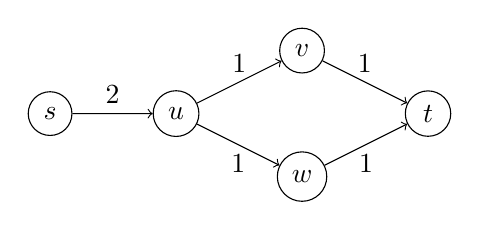
\begin{tikzpicture}[scale=0.8]
		\node[draw, circle] (S) at (0,2) {$s$};
		\node[draw, circle] (U) at (2,2) {$u$};
		\node[draw, circle] (W) at (4,1) {$w$};
		\node[draw, circle] (V) at (4,3) {$v$};
		\node[draw, circle] (T) at (6,2) {$t$};
		
		\path [->] (S) edge node[above] {$2$} (U);
		\path [->] (U) edge node[above] {$1$} (V);
		\path [->] (U) edge node[below] {$1$} (W);
		\path [->] (V) edge node[above] {$1$} (T);
		\path [->] (W) edge node[below] {$1$} (T);
		\end{tikzpicture}
	\end{subfigure}
	\begin{subfigure}{.45\textwidth}
		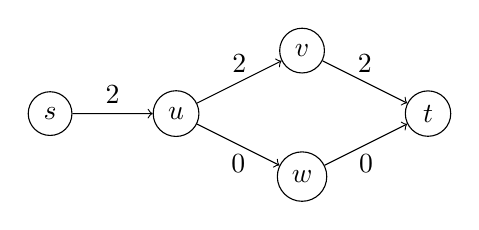
\begin{tikzpicture}[scale=0.8]
		\node[draw, circle] (S) at (0,2) {$s$};
		\node[draw, circle] (U) at (2,2) {$u$};
		\node[draw, circle] (W) at (4,1) {$w$};
		\node[draw, circle] (V) at (4,3) {$v$};
		\node[draw, circle] (T) at (6,2) {$t$};
		
		\path [->] (S) edge node[above] {$2$} (U);
		\path [->] (U) edge node[above] {$2$} (V);
		\path [->] (U) edge node[below] {$0$} (W);
		\path [->] (V) edge node[above] {$2$} (T);
		\path [->] (W) edge node[below] {$0$} (T);
		\end{tikzpicture}
	\end{subfigure}
	\caption{Zwei verschiedene schmale Flüsse derselben Instanz ohne Zurück\-setzen. Auf den Kanten steht der Flusswert; die Kapazitäten sind allesamt $1$.}
	\label{figure-thin-flows-not-unique}
\end{figure}

\begin{corollary}[Eindeutigkeit schmaler Flüsse]
	 Für eine Instanz von~$\problemThinFlow$ sind alle Lösungen auf den zurück\-setzen\-den Kanten sowie auf Kanten $vw$ mit $l_v \neq l_w$ identisch.
	 Dabei ist $(l_v)_{v\in V}$ die eindeutige Knotenauslastung.
\end{corollary}
\begin{proof}
	Da nach Lemma~\ref{lemma-node-congestion-unique} die Knotenauslastung $(l_v)_{v\in V}$ für jeden schmalen Fluss $f$ eindeutig ist, gilt $f_{vw} = u_{vw} l_w$ für $vw\in E_1$ nach~\ref{def-thin-flow-resetting-edge}.
	Für $vw\notin E_1$ betrachte man zunächst den Fall $l_v < l_w$.
	Nach Definition gilt $l_w \leq \max \{ l_v, f_{vw}/u_{vw} \}$, sodass man $f_{vw}/u_{vw} > l_v \geq 0$ folgern kann.
	Nach Lemma~\ref{lemma-equivalent-thin-flow} gilt also $f_{vw} = l_w u_{vw}$.
	Im Fall $l_v > l_w$ muss $f_{vw} = 0$ gelten, da sonst $l_w=\max\{ l_v, f_e/u_e \}$ gelten würde.
\end{proof}

\begin{theorem}[Existenz schmaler Flüsse]\label{thm-existence-thin-flow}
	Für jede Instanz von $\problemThinFlow$ existiert ein schmaler Fluss, falls im zugehörigen Netzwerk ein $s$-Fluss existiert.
\end{theorem}

Um die Existenz zu beweisen, benötigen wir zunächst den Fixpunktsatz von Kakutani.
Dazu führen wir die folgenden Begriffe ein:

\begin{definition}[Korrespondenz, Fixpunkt]
	Eine \emph{Korrespondenz} von einer Menge $A$ in eine Menge $B$ ist eine Abbildung $f: A \to \mathcal{P}(B)\setminus \{ \emptyset \}$ von $A$ in die Potenzmenge von $B$ ohne die leere Menge.
	Sind $A$ und $B$ topologische Räume, so nennt man $f$ \emph{abgeschlossen}, wenn die zugehörige Relation $R_f := \{ (a,b) \in A\times B \mid b\in f(a)  \}$ in der Produkttopologie abgeschlossen ist.

	Ein \emph{Fixpunkt} einer Korrespondenz $f: X \to \mathcal{P}$ ist ein Punkt $x\in X$ mit $x\in f(x)$.
\end{definition}

Nun lautet der Fixpunktsatz von Kakutani (siehe~\cite{Heuser1991Fix}):

\begin{satz}[Fixpunktsatz von Kakutani]\label{satz-kakutani}
	Seien $C\subseteq E$ eine nichtleere, konvexe und kompakte Teilmenge eines normierten Raumes $E$ und $f: C \to \mathcal{P}(C)$ eine abgeschlossene, konvexwertige Korrespondenz.
	Dann besitzt $f$ einen Fixpunkt.
\end{satz}

\begin{proof}[Beweis von Theorem~\ref{thm-existence-thin-flow}]
	Man betrachte die Menge $C$ aller $b$-Flüsse als Teilmenge des metrischen Raums $\R^E$.
	Nach Voraussetzung ist diese nichtleer, konvex, da für $f, g\in C, \lambda \in [0,1]$ der Fluss $\lambda f + (1-\lambda)g$ wieder die Flusserhaltung erfüllt, und kompakt, da jeder Fluss in $C$ aufgrund der Azyklizität in $s$-$v_i$-Wege zerlegbar ist, wodurch jede Kante maximal Fluss $b_s$ besitzen kann, sodass $C$ eine beschränkte Teilmenge von $\subseteq [0, b_s]^E$ ist.
	Außerdem ist $C$ abgeschlossen, da es die Lösungsmenge eines linearen Gleichungssystem ist.
	Auf $C$ definiere man die Korrespondenz
	\[
	\Gamma: C\to \mathcal{P}(C)\setminus\{ \emptyset \}, ~ f\mapsto \{ g\in C \mid \forall vw\in E: l_w < \rho_{vw}(l_v, f_{vw}) \implies g_{vw} = 0 \}.
	\]
	Dabei sei $l\in\R_{\geq 0}^V$ die zu $f$ gehörige Knotenauslastung.
	Diese Korrespondenz ist wohldefiniert, da $\Gamma(f)$ für jedes $f\in C$ nichtleer ist:
	Der Knoten $s$ kann im Graphen $G':= (V, E')$ mit $E':= \{ vw\in E \mid \rho_{vw}(l_v, f_{vw})=l_w \}$ jeden Knoten erreichen, da $G'$ azyklisch ist und jeder Knoten $w\neq s$ mindestens eine eingehende Kante mit $l_w = \rho_{vw}(l_v, f_{vw})$ besitzt. 
	Daher existiert ein $s$-$v$-Weg $P_v$ in $G'$ für alle $v\in V$ und der Fluss $\sum_{v\in V\setminus\{ s\}} b_v \cdot P_v$ ist in $\Gamma(f)$ enthalten.
	
	Für jedes $f\in C$ ist $\Gamma(f)$ konvex: Ist für $g, h\in \Gamma(f), \lambda\in [0,1]$ und eine Kante $vw\in E$ die Bedingung $l_w < \rho_{vw}(l_w, f_{vw})$ erfüllt, so gilt auch $\lambda g_{vw} + (1-\lambda) h_{vw} = 0$, womit $\lambda g + (1-\lambda)h$ im Bild $\Gamma(f)$ liegt.
	Des Weiteren ist $\Gamma$ abgeschlossen: 
	Sei eine konvergente Folge $((f^{n}, g^{n}))_{n\in\N}$ in $R_\Gamma$ mit Grenzwert $(f, g)$ gegeben.
	Die zu $f$ bzw. $f^n$ gehörigen Knotenauslastungen seien gegeben durch $l$ bzw. $l^n$.
	Angenommen, es gelte $l_w < \rho_{vw}(l_v, f_{vw})$.
	Da die Zuordnung $x'\mapsto l'$ eines $s$-Flusses auf seine Knotenauslastung nach Lemma~\ref{prop-congestion-labels-dijkstra} stetig ist, existiert ein $N\in\N$ mit $l_w^n<\rho_{vw}(l_v^n, f_{vw}^n)$ für alle $n\geq N$.
	Damit ist auch $g_{vw} = \lim_{n\to\infty} g_{vw}^n = 0$.
	
	Daher existiert nach dem Fixpunktsatz von Kakutani~\ref{satz-kakutani} ein Fixpunkt von $\Gamma$, welcher nach Lemma~\ref{lemma-equivalent-thin-flow} ein schmaler Fluss mit Zurücksetzen auf $E_1$ ist.
\end{proof}

\section{Effiziente Berechnung schmaler Flüsse}

Die Existenz schmaler Flüsse mit Zurücksetzen aus Theorem~\ref{thm-existence-thin-flow} suggeriert bereits einen exponentiellen Algorithmus, um einen solchen Fluss mit Wert $d$ zu berechnen:
Man rate die Menge $E'\subseteq E$ aller Kanten $vw$, die $l_w' = \rho_{vw}(l_v', x_{vw}')$ erfüllen, sowie für alle $vw\in E'\setminus E_1$ eine Binärzahl $\sigma_{vw}\in\{0,1\}$, die $\max\{ l_v', x_{vw}/u_{vw}\} = \sigma_{vw} l_v' + (1-\sigma_{vw}) x_{vw}/u_{vw}$ erfüllt.
Dann suche man einen zulässigen Punkt in folgendem Polyeder:
\begin{align*}
&	(x', l') \in \R_{\geq 0}^{E'\times V} \\
	\text{u.d.N.}\quad &
	x'(\delta^+(v)) - x'(\delta^-(v)) =
		\begin{cases}
			d, & \text{falls $v=s$},\\
			0, & \text{sonst,} 
		\end{cases} & \text{für $v\in V\setminus\{t \}$,} \\
	& l'_s = 0, \\
	& \begin{array}{@{}l}
		l_w' = \sigma_{vw} l_v' + (1-\sigma_{vw}) x'_{vw}/u_{vw}\\
		\sigma_{vw} l_v' + (1-\sigma_{vw}) x'_{vw}/u_{vw} \geq x'_{vw}/u_{vw}\\
		\sigma_{vw} l_v' + (1-\sigma_{vw}) x'_{vw}/u_{vw} \geq l_v'
	\end{array}
	& \text{für $vw\in E'\setminus E_1$},\\
	& l_w' = x'_{vw}/u_{vw} & \text{für $vw\in E_1$.}
\end{align*}
\todo{Genauerer Beweis}

\newcommand{\TFNP}{\mathbf{TFNP}}

Existiert solch ein Punkt $(x', l')$, so ist $x'$ nach Lemma~\ref{lemma-equivalent-thin-flow} ein schmaler Fluss mit Zurücksetzen auf $E_1$ mit zugehöriger Knotenbewertung $l'$.
Außerdem muss aufgrund der Existenz eines schmalen Flusses mindestens eine Wahl von $E'$ und $\sigma$ existieren, sodass der zugehörige Polyeder nichtleer ist.
\todo{Habe ich hier nicht das Problem, dass ich das nur für $\Q$ in polynomieller Zeit berechnen kann?}
Die Zulässigkeit eines solchen Polyeders kann in polynomieller Zeit beispielsweise durch die Ellipsoidmethode ermittelt werden. 
Daher liegt das Problem, zu einem Netzwerk $(V, E, u, s, t)$ einen schmalen $d$-Fluss mit Zurücksetzen auf $E_1\subseteq E$ zu finden, in der Komplexitätsklasse $\TFNP$:

\begin{definition}[Komplexitätsklasse $\TFNP$]
	Eine Relation $P(x,y)$ liegt in der Komplexitätsklasse $\TFNP$ genau dann, wenn es einen deterministischen, polynomiellen Algorithmus gibt, der entscheidet, ob $P(x,y)$ für zwei Kandidaten $x$ und $y$ gilt, und wenn für alle $x$ ein Kandidat $y$ existiert, dessen Kodierung polynomielle Größe in der Kodierungslänge von $x$ besitzt, sodass $P(x, y)$ gilt.
\end{definition}

In diesem Abschnitt wird ein polynomieller Algorithmus zur Berechnung von schmalen Flüssen ohne Zurücksetzen vorgestellt.

\begin{lemma}\label{lemma-thin-flows-without-resetting-have-minimal-congestion}
	Sei ein schmaler $b$-Fluss $f$ ohne Zurücksetzen mit zugehöriger Knotenauslastung $l$ gegeben.
	Dann ist $f$ ein $b$-Fluss minimaler Auslastung $q$ und für $E\neq\emptyset$ ist $X:=\{ v\in V \mid l_v < q \}$ ein dünnster Schnitt.
\end{lemma}
\begin{proof}
	Ist $b$ der Nullvektor -- wie im Fall $E=\emptyset$ --, ist $f$ der Nullfluss, da das Netzwerk azyklisch ist.
	
	Sei also $q>0$ die Auslastung von $f$ im Falle von $b\neq 0$.
	Nach Korollar~\ref{cor-thin-flows-max-node-label-equals-max-edge-label} genügt es zu
	zeigen, dass die Auslastung jeder ausgehenden Kante von $X$ bezüglich $f$ gerade $q$ beträgt und auf eingehenden Kanten von $X$ kein Fluss fließt.
	Wegen $l_s=0$ ist $s$ im Schnitt $X$ enthalten.
	Sei $vw\in\delta^+(X)$ eine ausgehende Kante.
	Dann gilt $l_v < l_w = q $ und nach Proposition~\ref{prop-congestion-labels-dijkstra} auch $q = l_w \leq \rho_{vw}(l_v, f_{vw}) = f_{vw} / u_{vw}$.
	Da $q$ eine obere Schranke an $f_{vw}/u_{vw}$ ist, gilt also $f_{vw}/u_{vw} = q$.
	Für eine eingehende Kante $vw\in\delta^-(X)$ gilt $\rho_{vw}(l_v, f_{vw})\geq l_v > l_w$ und somit muss nach Lemma~\ref{lemma-equivalent-thin-flow} der Fluss $f$ auf der Kante $vw$ verschwinden.
\end{proof}

\begin{definition}
	Seien $\mathcal{I}:=(V, E, u, b)$ eine $b$-Fluss-Instanz und $X\subseteq V$ ein dünnster Schnitt mit Auslastung $q$.
	Dann heißt $\mathcal{I}[X] := (X, E[X], u[X], b[X])$ die \emph{durch $X$ induzierte Teilinstanz von $\mathcal{I}$},
	wobei $E[X] := \{ vw \in E \mid v, w \in X \}$ als die Menge der Kanten zwischen Knoten in $X$, $u[X]$ als die Einschränkung von $u$ auf $E[X]$ und $b[X]$ durch \[
	b[X]_v := b_v - u(\delta^+_E(v)\cap\delta^+_E(X)) q \quad \text{für $v\in X$}
\] definiert ist.
\end{definition}

Man bemerke, dass $b[X]_v \leq b_v$ für $v\in X$ erfüllt und $b[X]$ ein zulässiger Balancevektor ist: \[
	\sum_{v\in X} b[X]_v = b(X) - u(\delta^+_E(X)) q = 0
\]

\begin{proposition}\label{prop-restricted-minimal-flow-is-b-flow-on-induced-instance}
	Ist $f$ ein $b$-Fluss minimaler Auslastung einer $b$-Fluss-Instanz $(V, E, u, b)$, so ist die Einschränkung $f':=f_{\mid E[X]}$ ein $b[X]$-Fluss der induzierten Instanz $(X, E[X], u[X], b[X])$ für jeden dünnsten Schnitt $X$.
	Ist $f$ sogar ein $s$-Fluss mit Knotenauslastung $l$ und $b_s > 0$, so stimmt die Einschränkung von $l$ auf $X$ mit der Knotenauslastung $l'$ vom $s$-Fluss $f'$ überein.
\end{proposition}
\begin{proof}
	Nach Korollar~\ref{cor-easy-characterization-sparsest-cut} gelten $f_{e}/u_{e}=q$ für $e\in\delta^+(X)$ und $f_{e} = 0$ für $e\in\delta^-(X)$.
	Daher kann man zeigen, dass $f'$ ein $b[X]$-Fluss ist, denn für alle $v\in X$ gilt:
	\begin{align*}
	f'(\delta^+_{E[X]}(v)) - f'(\delta^-_{E[X]}) &= f(\delta^+_E(v)) - f(\delta^-_E(v)) - f(\delta^+_{E[X]}(v)\cap\delta^+_{E[X]}(X)) \\
	&= b_v - u(\delta^+_{E[X]}(v)\cap\delta^+_{E[X]}(X))q = b[X]_v.
	\end{align*}
	Sei nun $f$ sogar ein $s$-Fluss mit $b_s > 0$, wodurch $s$ in $X$ enthalten ist.
	Sei $v\in X$ gegeben.
	Da jeder $s$-$v$-Pfad in $(X, E')$ auch in $(V, E)$ enthalten ist, gilt bereits $l'_v\leq l_v$.
	Außerdem liegt jeder $s$-$v$-Pfad in $(V, E)$ mit positivem Fluss bezüglich $f$ auch komplett in $(X, E')$, da $f$ auf $\delta^-_E(X)$ verschwindet.
	Daraus folgt $l'_v \geq l_v$.
\end{proof}

Daher kann man bereits erkennen, dass ein schmaler Fluss ohne Zurücksetzen eingeschränkt auf eine durch einen dünnsten Schnitt induzierte Teilinstanz wieder ein schmaler Fluss ist.
Das Ziel ist es nun, aus einem schmalen Fluss der Teilinstanz einen schmalen Fluss auf der ursprünglichen Instanz zu konstruieren.

\begin{lemma}\label{lemma-flow-minimal-congestion-sparsest-cut-then-outside-X-congestion-q}
	Seien ein $s$-Fluss $f$ minimaler Auslastung $q^*$ mit zugehöriger Knotenauslastung $l$ und ein dünnster Schnitt $X$ in einem Netzwerk ohne zurücksetzende Kanten gegeben.
	Für alle $v\in V\setminus X$ hat jeder $s$-$v$-Pfad $P$ Auslastung $q^*=l_v$.
\end{lemma}
\begin{proof}
	Ist $b$ der Nullvektor, so ist $f$ der Nullfluss und $l_v = 0$ für alle $v\in V$.
	Sonst ist $s$ in $X$ enthalten und für alle $v\in V\setminus X$ enthält jeder $s$-$v$-Pfad mindestens eine Kante, die $X$ verlässt und nach Korollar~\ref{cor-easy-characterization-sparsest-cut} Auslastung $q^*$ besitzt.
	Da das Netz keine zurücksetzenden Kanten hat, beträgt die Auslastung also $\max_{e\in P} f_e / u_e = q^*$.
\end{proof}

\begin{corollary}
	Seien ein $s$-Fluss $f$ minimaler Auslastung sowie ein dünnster Schnitt $X$ auf einem Netzwerk ohne zurücksetzende Kanten gegeben.
	Ist $f'$ ein schmaler Fluss ohne Zurücksetzen auf der durch $X$ induzierten Teilinstanz, so ist \[
		g_e := \begin{cases}
			f'_e, & \text{falls $e\in E[X]$,} \\
			f_e, & \text{falls $e\in E\setminus E[X]$,}
		\end{cases}
	\] ein schmaler Fluss ohne Zurücksetzen auf der ursprünglichen Instanz.
\end{corollary}
\begin{proof}
	Es ist leicht zu sehen, dass $g$ ein $s$-Fluss minimaler Auslastung ist:
	Für einen Knoten $v \in V\setminus X$ ist $g(\delta^+_E(v)) - g(\delta^-_E(v)) = f(\delta^+_E(v)) - g(\delta^-_E(v)) = b_v$ und für $v\in X$ gilt
	\begin{align*}
	g(\delta^+_E(v)) - g(\delta^-_E(v)) =& f'(\delta^+_{E[X]}(v))  - f'(\delta^-_{E[X]}(v))  \\
	&+ f(\delta^+_E(v)\cap\delta^+_E(X)) - f(\delta^-_E(v)\cap\delta^-_E(X)) = b_v
	\end{align*}

	Sei ein $s$-$v$-Pfad $P$ mit positivem Fluss gegeben.
	Ist $v$ nicht in $X$, so hat $P$ nach Lemma~\ref{lemma-flow-minimal-congestion-sparsest-cut-then-outside-X-congestion-q} Auslastung $l_v$.
	Ist $v$ in $X$ enthalten, muss $P$ entlang Kanten innerhalb von $X$ laufen, da $g$ auf eingehenden Kanten von $X$ verschwindet.
	Nach Proposition~\ref{prop-restricted-minimal-flow-is-b-flow-on-induced-instance} stimmt die Auslastung von $v$ bezüglich der Einschränkung von $f$ mit der Auslastung von $v$ bezüglich $f$ überein, sodass auch die Auslastung von $P$ mit der Auslastung von $v$ bezüglich $f$ übereinstimmen.
\end{proof}

\begin{algorithm}
\caption{Berechnung eines schmalen Flusses ohne Zurücksetzen}
\label{algorithm-computation-thin-flow-without-resetting}
\begin{algorithmic}[1]
	\Function{ThinFlow}{$V, E, u, b, s$}
	\If{$b_s = 0$}
	\State\Return $0^E$
	\Else 
	\State Berechne $s$-Fluss $f$ minimaler Auslastung und dünnsten Schnitt $X$
	\State $f' \gets $ \Call{ThinFlow}{$X, E[X], u[X], b[X], s$}
	\ForAll{$e\in E[X]$} \State $f_e \gets f'_e$ \EndFor
	\State\Return $f$
	\EndIf
	\EndFunction
\end{algorithmic}
\end{algorithm}

Dies bildet die Grundlage des polynomiellen Algorithmus'~\ref{algorithm-computation-thin-flow-without-resetting} zur Berechnung von schmalen Flüssen ohne Zurücksetzen.
